% !TEX program = xelatex
\documentclass[10.5pt,a4paper,headings=small,abstract=false]{scrartcl}

% ---------- Tipografía: TeX Gyre Pagella (texto, tablas y fórmulas), Figtree (títulos y rótulos)
\usepackage{fontspec}
\usepackage{polyglossia}
\setmainlanguage{spanish}
\addto\captionsspanish{\renewcommand{\tablename}{Tabla}\renewcommand{\figurename}{Figura}\renewcommand{\refname}{Referencias}}
\setmainfont{texgyrepagella}[Extension=.otf,UprightFont=*-regular,BoldFont=*-bold,ItalicFont=*-italic,BoldItalicFont=*-bolditalic,Numbers={Lining,Monospaced}]
\setsansfont{Figtree}[Path=/home/diego/.fonts/,Extension=.ttf,UprightFont=*-Regular,BoldFont=*-Bold,ItalicFont=*-ItalicRegular,BoldItalicFont=*-Italic,Numbers={Lining,Monospaced}]
\usepackage{unicode-math}
\setmathfont{texgyrepagella-math.otf}[Path=/usr/share/texmf-dist/fonts/opentype/public/tex-gyre-math/]
\usepackage{microtype}

% ---------- Color
\usepackage{xcolor}
\definecolor{acento}{HTML}{0E5E5C}
\definecolor{acentoclaro}{HTML}{EEF5F4}
\definecolor{ambar}{HTML}{B8741F}
\definecolor{tinta}{HTML}{22343A}
\definecolor{gris}{HTML}{5F6F74}
\definecolor{filete}{HTML}{B9CFCD}

% ---------- Página y ritmo
\usepackage[a4paper,left=2.7cm,right=2.7cm,top=2.7cm,bottom=2.7cm]{geometry}
\usepackage{setspace}
\setstretch{1.0}
\setlength{\parindent}{0pt}
\setlength{\parskip}{0.4em}
\raggedbottom
\setlength{\textfloatsep}{10pt plus 2pt minus 2pt}\setlength{\floatsep}{8pt plus 2pt minus 2pt}\setlength{\intextsep}{8pt plus 2pt minus 2pt}
\setlength{\emergencystretch}{3em}
\tolerance=1200
\renewcommand{\topfraction}{0.9}\renewcommand{\floatpagefraction}{0.82}\setcounter{totalnumber}{4}
\usepackage{fancyhdr}
\pagestyle{fancy}\fancyhf{}
\renewcommand{\headrulewidth}{0pt}
\fancyhead[L]{\color{gris}\footnotesize Estadías hospitalarias en FONASA, 2020}
\fancyfoot[C]{\color{gris}\footnotesize\thepage}
\fancypagestyle{plain}{\fancyhf{}\fancyfoot[C]{\color{gris}\footnotesize\thepage}\renewcommand{\headrulewidth}{0pt}}

% ---------- Títulos
\setkomafont{disposition}{\sffamily\bfseries\color{acento}}
\setkomafont{section}{\sffamily\bfseries\color{acento}\Large}
\setkomafont{subsection}{\sffamily\bfseries\color{acento}\large}
\setkomafont{subsubsection}{\sffamily\bfseries\color{tinta}\normalsize}
\RedeclareSectionCommand[beforeskip=1.7em plus .3em minus .2em,afterskip=0.5em]{section}
\RedeclareSectionCommand[beforeskip=1.1em plus .2em minus .1em,afterskip=0.35em]{subsection}
\setkomafont{captionlabel}{\bfseries\color{acento}\footnotesize}
\setkomafont{caption}{\footnotesize\color{tinta}}
\color{tinta}

% ---------- Paquetes
\usepackage{amsmath}
\usepackage{graphicx}
\usepackage{booktabs}
\usepackage{colortbl}
\usepackage{array}
\usepackage{tabularx}
\usepackage{float}
\usepackage{caption}
\usepackage{tikz}
\usetikzlibrary{arrows.meta,positioning}
\usepackage{url}\urlstyle{same}
\usepackage[colorlinks=true,linkcolor=acento,citecolor=acento,urlcolor=acento]{hyperref}
\usepackage[authoryear,round]{natbib}
\setcitestyle{aysep={,}}
\setlength{\bibhang}{1.27cm}
\captionsetup{font=small,justification=raggedright,singlelinecheck=false,labelsep=period,skip=6pt}
\captionsetup[table]{position=above}
\captionsetup[figure]{position=above}
\renewcommand{\arraystretch}{1.2}
\arrayrulecolor{filete}
\setlength{\heavyrulewidth}{0.9pt}\setlength{\lightrulewidth}{0.4pt}

\newcommand{\fuente}{\par\vspace{0.3em}{\footnotesize\color{gris}Fuente: DEIS, MINSAL, egresos hospitalarios 2020; elaboración propia.\par}}
\newcolumntype{Y}{>{\raggedright\arraybackslash}X}
\newcommand{\cie}{\mbox{CIE-10}}
\newcommand{\pct}{\,\%}
\newcommand{\filas}{\rowcolors{2}{white}{acentoclaro}}

\title{Factores asociados a la duración de la estadía y a las estadías prolongadas en beneficiarios FONASA, Chile 2020}
\author{Proyecto de Análisis de Datos (IIP316W-1)}
\date{10 de noviembre de 2026}

\begin{document}

% ---------- Portada compacta
{\raggedright
{\sffamily\bfseries\color{acento}\fontsize{21}{25}\selectfont Factores asociados a la duración de la estadía y a las estadías prolongadas en beneficiarios FONASA, Chile 2020\par}
\vspace{0.9em}
{\color{gris}\small Proyecto de Análisis de Datos (IIP316W-1) \quad·\quad 10 de noviembre de 2026\par}
\vspace{0.4em}
{\color{filete}\rule{\textwidth}{0.6pt}}\par}
\vspace{0.4em}

{\sffamily\bfseries\color{acento}\large Resumen}\par\vspace{-0.2em}
Estudiamos los 968.098 egresos FONASA de 2020 publicados por el DEIS. Las estadías de más de 15 días son el 9,4\pct{} de los egresos y usan el 47,1\pct{} de los días-cama. Evaluamos qué factores clínicos, demográficos y del sistema de salud se asocian con la duración y con esas estadías, y qué tan grande es cada asociación. Usamos la base completa, así que las medidas de ajuste describen esta población. Una regresión lineal múltiple de $\ln$(días) explica el 19,8\pct{} de la variación ($R^2$ ajustado $=0{,}198$). El capítulo \cie{} es el factor con mayor aporte ($\eta^2$ parcial $=0{,}074$), seguido del tipo de establecimiento ($0{,}041$) y de la edad ($0{,}035$). Frente a los egresos fuera de la red, los del SNSS tienen una media geométrica de días 70,0\pct{} mayor y un OR de 2,54 para la estadía prolongada. Sexo, cirugía, condición de egreso y región son significativos, pero su aporte es pequeño. Como la base no trae gravedad ni identificadores de paciente y hospital, las asociaciones no son causales.

{\small\color{gris}\textbf{Palabras clave:} estadía hospitalaria, FONASA, regresión lineal múltiple, regresión logística, tamaño del efecto, \cie.\par}

% =====================================================================
\section{Introducción}

La gestión de camas depende de cuánto dura cada hospitalización, y esa duración es muy desigual. En los egresos FONASA de 2020 la mitad dura 3 días o menos, pero las estadías de más de 15 días ocupan casi la mitad de los días-cama. Saber qué se asocia a esas estadías ayuda a entender dónde se concentra el uso de camas.

La pregunta de investigación es:

\begin{quote}
\emph{¿Qué factores clínicos, demográficos y del sistema de salud se asocian con la duración de la estadía y con las estadías prolongadas (más de 15 días) en los egresos FONASA de Chile en 2020?}
\end{quote}

Consideramos prolongada una estadía de más de 15 días, que corresponde al percentil 90 de la duración. Las hipótesis son:

\begin{itemize}\setlength\itemsep{0pt}
\item $H_0$: la duración de la estadía y la ocurrencia de estadías prolongadas no se asocian con los factores clínicos, demográficos ni del sistema de salud.
\item $H_1$: al menos uno de esos factores se asocia con la duración de la estadía o con la ocurrencia de estadías prolongadas.
\end{itemize}

Formulamos además una $H_1$ por grupo de factores, que dice que los factores del grupo se asocian con la duración y con la estadía prolongada.

\begin{itemize}\setlength\itemsep{0pt}
\item $H_{1a}$ (clínicos): capítulo del diagnóstico (\cie), cirugía y condición de egreso.
\item $H_{1b}$ (demográficos): edad y sexo. Nacionalidad y etnia entran solo como análisis de sensibilidad. Esperamos más días a mayor edad.
\item $H_{1c}$ (sistema de salud): tipo de establecimiento y región.
\end{itemize}

% =====================================================================
\section{Revisión de literatura}

Los Grupos Relacionados por el Diagnóstico (GRD) agrupan a los pacientes según su diagnóstico y sus procedimientos, porque esas dos cosas explican buena parte de los recursos que consume una hospitalización y de lo que dura \citep{fetter1980}. \citet{freitas2012} analizaron 9 millones de hospitalizaciones en Portugal y encontraron que la edad y el tipo de hospital seguían asociados a las estadías extremas dentro de un mismo GRD. Por eso no nos quedamos solo con el diagnóstico: incluimos factores del paciente y del establecimiento.

La revisión sistemática de \citet{lequertier2021} muestra que la regresión es el método más usado para modelar la duración de la estadía. Aquí la usamos para describir asociaciones. Para revisar los supuestos del estimador de mínimos cuadrados ordinarios seguimos a \citet{rodriguez2017}.

Con bases de este tamaño casi cualquier diferencia sale significativa. \citet{lin2013} recomiendan reportar el tamaño del efecto junto con el valor-$p$, y nosotros lo interpretamos con los umbrales de \citet{cohen1988}. En las pruebas no paramétricas, el tamaño del efecto de dos grupos es la correlación biserial de rangos \citep{kerby2014}. \citet{raftery1995} plantea el mismo problema para la selección de modelos: con muestras grandes, elegir variables por su valor-$p$ deja variables que casi no aportan. Propone el criterio de información bayesiano (BIC; \citealt{schwarz1978}), que usamos para decidir qué variables entran a los modelos.

En Chile, \citet{olivares2020} estudió las estadías largas, pero solo en adultos mayores. No encontramos un trabajo que mire a la vez factores clínicos, demográficos y del sistema de salud en el total de egresos FONASA, ni uno sobre 2020, el primer año de la pandemia. Como la base abierta no trae peso GRD ni gravedad, la pregunta de fondo es cuánto de la duración se asocia con las variables que sí están disponibles.

% =====================================================================
\section{Metodología}

\subsection{Diseño del estudio}

Es un estudio observacional retrospectivo y analítico. Describe la distribución de la duración, contrasta las hipótesis con pruebas de asociación y estima asociaciones ajustadas con modelos de regresión. Todos los modelos se estiman con los 968.098 egresos y sus medidas de ajuste ($R^2$, devianza, pseudo-$R^2$) describen esta población. La figura~\ref{fig:diagrama} resume el flujo.

\begin{figure}[!htb]
\centering
\caption{Diagrama metodológico.}
\label{fig:diagrama}
\begin{tikzpicture}[node distance=0.25cm, every node/.style={font=\footnotesize\sffamily},
 caja/.style={draw=acento, rounded corners=2pt, minimum width=2.4cm, minimum height=1.25cm, text width=2.25cm, align=center, fill=acentoclaro},
 flecha/.style={-{Stealth[length=1.8mm]}, thick, color=acento}]
\node[caja] (a) {\textbf{Problema}\\ duración y estadía prolongada};
\node[caja, right=of a] (b) {\textbf{Datos}\\ DEIS 2020, 968.098 egresos};
\node[caja, right=of b] (c) {\textbf{Procesamiento}\\ filtros, variables, exploración};
\node[caja, right=of c] (d) {\textbf{Asociaciones}\\ pruebas de a pares, tamaño del efecto};
\node[caja, right=of d] (e) {\textbf{Modelamiento}\\ lineal, logístico, sensibilidad};
\foreach \i/\j in {a/b,b/c,c/d,d/e} \draw[flecha] (\i)--(\j);
\end{tikzpicture}
{\footnotesize\color{gris}Fuente: elaboración propia.\par}
\end{figure}

\subsection{Datos}

La fuente son los egresos hospitalarios 2020 del DEIS-MINSAL (datos abiertos). Usamos solo egresos FONASA (\texttt{PREVISION = 1}) con estadías de hasta 365 días, como en el Avance 1. Excluimos 397 egresos (0,04\pct{}) de más de un año por esa regla de depuración. El máximo es de 16.598 días, unos 45 años, y la duración por sí sola no demuestra que todos sean errores de registro. Quedan 968.098 egresos, dentro del rango pedido de 700.000 a 1.000.000. La unidad de análisis es el egreso, no el paciente.

\subsection{Variables}

La base trae 18 columnas. Revisamos cada una con tres condiciones: que su significado esté en el diccionario del DEIS o se pueda verificar con los datos, que varíe entre egresos y que no repita otra columna. Quedaron nueve variables candidatas y dos respuestas (tabla~\ref{tab:vars}). \texttt{DIAG2} se descarta porque está vacía en el 90,2\pct{} de los egresos. \texttt{COMUNA\_RESIDENCIA} repite la región con 344 categorías. \texttt{PROCED} no está en el diccionario y no pudimos verificar qué registra. \texttt{INTERV\_Q} tampoco está, pero su codificación calza con cirugía: por ejemplo, vale 1 en el 97\pct{} de las cesáreas.

\begin{table}[!htb]
\centering\footnotesize\filas
\caption{Variables del estudio.}
\label{tab:vars}
\begin{tabularx}{\textwidth}{>{\raggedright\arraybackslash}p{2.9cm} >{\raggedright\arraybackslash}p{3.7cm} >{\raggedright\arraybackslash}p{2.6cm} Y}
\toprule
Variable & Columna & Tipo & Justificación \\
\midrule
Días de estada & \texttt{DIAS\_ESTADA} & Numérica & Respuesta de la regresión lineal (en $\ln$) \\
Estadía prolongada & días $>15$ & Categórica (Sí/No) & Respuesta del chi-cuadrado y de la logística \\
Capítulo \cie & \texttt{DIAG1} & Categórica (21) & Aproxima la gravedad, porque no hay peso GRD \\
Cirugía & \texttt{INTERV\_Q} & Categórica (Sí/No) & Distingue casos quirúrgicos de médicos \\
Condición de egreso & \texttt{CONDICION\_EGRESO} & Categórica (vivo/fallecido) & Los fallecidos suelen ser casos graves \\
Edad & \texttt{GRUPO\_EDAD} & Numérica (punto medio) & Más edad, más días \citep{freitas2012} \\
Sexo & \texttt{SEXO} & Categórica & Variable demográfica básica \\
Nacionalidad & \texttt{GLOSA\_PAIS\_ORIGEN} & Categórica (2) & Revisar si el origen cambia la duración \\
Etnia & \texttt{ETNIA} & Categórica (Sí/No) & Revisar pertenencia a pueblo originario \\
Establecimiento & \texttt{PERTENENCIA\_...} & Categórica (SNSS/No SNSS) & Tipo de hospital \citep{freitas2012} \\
Región & \texttt{REGION\_RESIDENCIA} & Categórica (16) & Acceso y oferta de camas \\
\bottomrule
\end{tabularx}
\fuente
\end{table}

La condición de egreso se conoce recién al alta, así que los modelos no sirven como herramienta de decisión al ingreso.

\subsection{Asociaciones de a pares}

Usamos $\alpha=0{,}05$. Verificamos la normalidad de las variables numéricas con Shapiro--Wilk (en una muestra de 5.000 egresos, porque con más datos su valor-$p$ deja de ser exacto), Kolmogorov--Smirnov con corrección de Lilliefors y Anderson--Darling. Como la normalidad se rechaza, usamos pruebas no paramétricas: Spearman para numérica contra numérica, Mann--Whitney U (dos grupos) y Kruskal--Wallis (tres o más, con comparaciones por pares de Mann--Whitney y corrección de Holm) para numérica contra categórica, y chi-cuadrado de independencia con V de Cramér para categórica contra categórica. Hacemos 20 pruebas. Con la corrección de Bonferroni el nivel sería $0{,}05/20=0{,}0025$ y ninguna decisión cambia: las 18 pruebas de asociación tienen $p<0{,}0002$ y las de normalidad $p<0{,}001$.

Los umbrales de \citet{cohen1988} para efecto pequeño, mediano y grande son 0,1, 0,3 y 0,5 en $\rho$, $r$ y $V$ de Cramér, y 0,01, 0,06 y 0,14 en $\varepsilon^2$ y $\eta^2$.

\subsection{Selección de variables}

En el Avance 1 ajustamos un modelo lineal de $\ln$(días) con las nueve candidatas y eliminamos hacia atrás según el BIC,
\[
\mathrm{BIC}=n\,\ln\!\left(\frac{\mathrm{SCR}}{n}\right)+k\,\ln n,
\]
donde SCR es la suma de cuadrados de los residuos y $k$ el número de coeficientes. Cada coeficiente cuesta $\ln(968.098)\approx 13{,}8$. Para una variable de un coeficiente, eso equivale a exigir un $F$ parcial mayor que 13,8 en vez del 3,84 que pide $p<0{,}05$ \citep{raftery1995}. Quedaron siete variables: capítulo, cirugía, condición de egreso, edad, sexo, establecimiento y región. Nacionalidad y etnia salieron, y revisamos su incorporación como sensibilidad (sección~\ref{sec:sens}).

\subsection{Regresión lineal múltiple}

Estimamos por mínimos cuadrados ordinarios el modelo M3, con los siete factores a la vez para describir la asociación de cada uno con los demás constantes:
\begin{multline*}
\ln(\text{días}_i)=\beta_0+\sum_c\gamma_c\,\text{capítulo}_{ic}+\beta_1\,\text{cirugía}_i+\beta_2\,\text{fallecido}_i+\beta_3\,\text{edad}_{c,i}\\
+\beta_4\,\text{edad}_{c,i}^2+\beta_5\,\text{hombre}_i+\beta_6\,\text{SNSS}_i+\sum_r\delta_r\,\text{región}_{ir}+\varepsilon_i .
\end{multline*}
La referencia de capítulo es K00--K93 (digestivo): tiene hombres y mujeres y una mediana de 2 días, así que los demás capítulos se leen como diferencias respecto de un egreso corto y habitual. No usamos O00--O99 porque solo tiene mujeres. La referencia de región es la Región Metropolitana, el sexo de referencia es mujer y la edad está centrada en su media (45,01 años).

Como el modelo describe la media condicional de $\ln$(días), su exponencial es una media geométrica condicional. Por eso interpretamos $100\,(e^{\beta}-1)\pct{}$ como el cambio porcentual en la media geométrica de los días.

Para ver cuánto aporta cada bloque ajustamos cuatro modelos anidados: M0 (solo intercepto), M1 (bloque clínico), M2 (M1 más edad, edad$^2$ y sexo) y M3 (M2 más establecimiento y región). Comparamos BIC, $F$ parcial y $\eta^2$ parcial. El $\eta^2$ parcial de un bloque o factor es la parte de la variación que quedaba sin explicar y que su inclusión explica:
\[
\eta^2_{\text{parcial}}=\frac{R^2_{\text{con}}-R^2_{\text{sin}}}{1-R^2_{\text{sin}}}.
\]
Como el aporte secuencial depende del orden en que entran los bloques, también retiramos cada factor de M3 y medimos cuánto baja el $R^2$. Un factor es relevante si, además de significativo, su $\eta^2$ parcial es de al menos 0,01. Es un criterio orientativo: con casi un millón de egresos, el valor-$p$ no distingue entre efectos grandes y pequeños.

\subsection{Regresión logística}

Para la estadía prolongada (más de 15 días) ajustamos modelos logísticos anidados con los mismos siete factores, con la edad en tramos (L1: factores clínicos; L2: más edad y sexo; L3: más establecimiento y región). Un coeficiente se interpreta como razón de odds (OR): cuánto se multiplican los odds de una estadía prolongada cuando el factor cambia, con lo demás constante. Medimos el aporte con la razón de verosimilitud y con la caída del pseudo-$R^2$ de McFadden al retirar cada factor.

\subsection{Supuestos y sensibilidad}

Revisamos la forma funcional, el rango de la matriz de diseño, la multicolinealidad con el VIF, la heterocedasticidad y la distribución de los residuos. Como la varianza de los residuos no es constante, reportamos además errores estándar robustos HC3 para los coeficientes de M3. La exogeneidad, $E(\varepsilon\mid X)=0$, es un supuesto, y la independencia no se puede verificar con esta base porque no identifica pacientes ni hospitales. Como análisis de sensibilidad comparamos M3 con tres alternativas: M4 cambia edad y edad$^2$ por los 11 tramos de edad; M5 agrega la interacción capítulo $\times$ establecimiento; M6 agrega tramo de edad $\times$ establecimiento. También agregamos nacionalidad y etnia a M3. Por último, repetimos la selección con un procedimiento forward por BIC.

% =====================================================================
\section{Resultados}

\subsection{Descripción y depuración}

Los días de estada tienen media 6,70 y mediana 3 (Q1 $=2$, Q3 $=7$). La desviación estándar (12,79) casi duplica la media y la asimetría es 9,04: la mayoría dura pocos días y unos pocos duran muchísimo (tabla~\ref{tab:desc} y figura~\ref{fig:dist}). En $\ln$(días) la asimetría baja a 0,68 y la media queda cerca de la mediana, por eso modelamos el logaritmo.

\begin{table}[!htb]
\centering\small\filas
\caption{Estadísticos descriptivos ($n=968.098$).}
\label{tab:desc}
\begin{tabular}{lrrrrr}
\toprule
Variable & Media & Mediana & Desv. est. & Asimetría & RIC \\
\midrule
Días de estada & 6,70 & 3,00 & 12,79 & 9,04 & 5,00 \\
$\ln$(días) & 1,25 & 1,10 & 1,04 & 0,68 & 1,25 \\
Edad (años) & 45,01 & 44,50 & 24,29 & 0,01 & 40,00 \\
\bottomrule
\end{tabular}
\fuente
\end{table}

\begin{figure}[!htb]
\centering
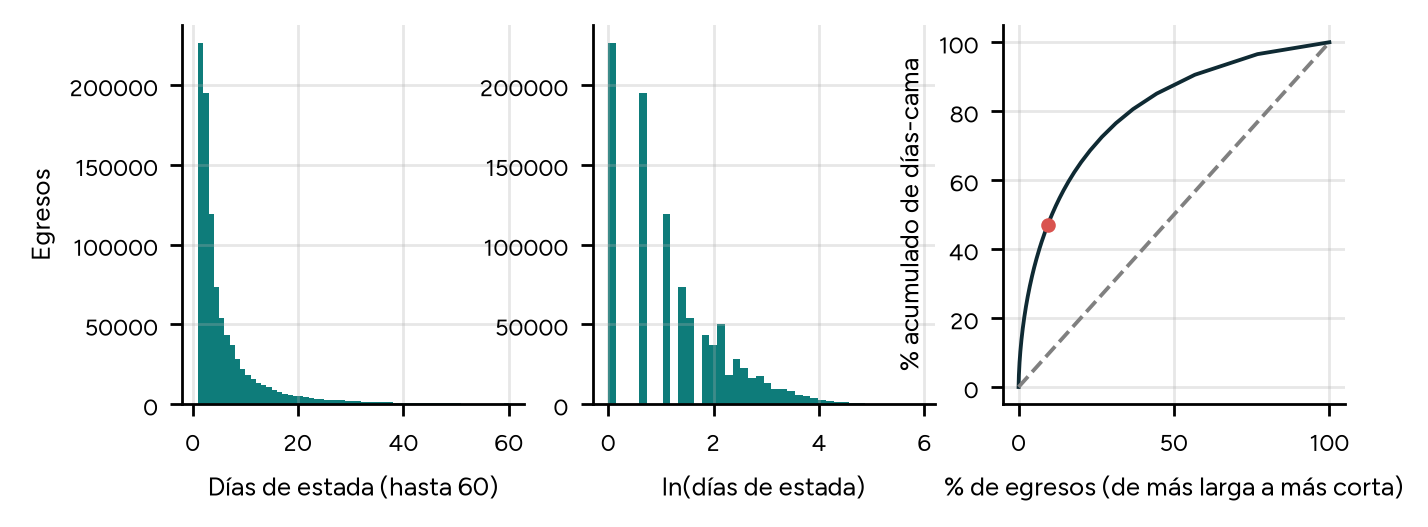
\includegraphics[width=0.92\textwidth]{figs/avance2_distribucion.png}
\caption{Distribución de los días de estada (izquierda, recortada a 60 días), de $\ln$(días) (centro) y curva de concentración de los días-cama (derecha). Los egresos de más de 15 días son el 9,4\pct{} y usan el 47,1\pct{} de los días-cama.}
\label{fig:dist}
\fuente
\end{figure}

El 81,8\pct{} de los egresos son de establecimientos del SNSS y el 60,0\pct{} son de mujeres. Los capítulos más frecuentes son embarazo, parto y puerperio (O00--O99, 20,4\pct{}), digestivo (K00--K93, 13,8\pct{}) y traumatismos (S00--T98, 9,8\pct{}). La respuesta y las siete variables explicativas no tienen valores nulos, así que no imputamos ni eliminamos egresos.

Con el criterio de Tukey, el límite superior de los días es 14,5 y lo superan 99.978 egresos (10,33\pct{}). Con los 397 egresos de más de 365 días, la media subiría de 6,70 a 7,29 y la desviación estándar de 12,79 a 59,74, sin cambiar la mediana (3) ni el MAD (2).

\subsection{Normalidad y asociaciones de a pares}

Las tres pruebas rechazan la normalidad de los días y de la edad (Shapiro--Wilk y Lilliefors con $p<0{,}001$; Anderson--Darling con $p=0{,}01$, el valor más bajo que informa \texttt{scipy}). Por eso usamos pruebas no paramétricas.

La edad se relaciona con los días con $\rho=0{,}25$ ($p<0{,}001$): a mayor edad la estadía tiende a ser más larga, con un efecto pequeño. La mediana sube de 2 días en adultos jóvenes a 6 días desde los 80 años, con la excepción de los menores de un año (mediana de 4 días). Con Mann--Whitney y Kruskal--Wallis todos los factores rechazan $H_0$ ($p<0{,}001$), pero con efectos distintos. El establecimiento ($r=-0{,}37$, mediano) y el capítulo ($\varepsilon^2=0{,}12$, mediano) son los mayores; condición de egreso, cirugía y sexo tienen efectos pequeños; nacionalidad, etnia y región son despreciables (figura~\ref{fig:biv}). En el chi-cuadrado sobre la estadía prolongada, todas las frecuencias esperadas superan 5 (la menor es 175) y la asociación más fuerte es la del capítulo ($V=0{,}25$, de 0,9\pct{} de prolongadas en partos a 35,6\pct{} en trastornos mentales). La edad tiene forma de U: 15,4\pct{} de prolongadas en menores de un año, 3,5\pct{} entre 20 y 29 años y 15,4\pct{} entre 70 y 79. La tabla~\ref{tab:resumen} resume las pruebas.

\begin{table}[!htb]
\centering\footnotesize\filas
\caption{Resumen de las pruebas de a pares. Las pruebas de asociación tienen $p<0{,}001$.}
\label{tab:resumen}
\begin{tabularx}{\textwidth}{>{\raggedright\arraybackslash}p{3.0cm} >{\raggedright\arraybackslash}p{2.0cm} >{\raggedright\arraybackslash}p{3.0cm} Y}
\toprule
Variable 1 & Variable 2 & Prueba & Conclusión \\
\midrule
Días y edad & Normalidad & Shapiro--Wilk, Lilliefors, A--D & No son normales \\
Edad & Días & Spearman & $\rho=0{,}25$ (pequeño) \\
Establecimiento & Días & Mann--Whitney U & SNSS más largas ($r=-0{,}37$, mediano) \\
Capítulo \cie & Días & Kruskal--Wallis + Holm & Mediana de 1 a 9 días ($\varepsilon^2=0{,}12$, mediano) \\
Condición de egreso & Días & Mann--Whitney U & Fallecidos más largas ($r=-0{,}29$, pequeño) \\
Cirugía & Días & Mann--Whitney U & Sin cirugía más largas ($r=0{,}22$, pequeño) \\
Sexo & Días & Mann--Whitney U & Hombres más largas ($r=0{,}14$, pequeño) \\
Nacionalidad, etnia & Días & Mann--Whitney U & Despreciable ($r=0{,}06$ y $-0{,}02$) \\
Región & Días & Kruskal--Wallis + Holm & Despreciable ($\varepsilon^2=0{,}002$) \\
Capítulo \cie & Prolongada & Chi-cuadrado & $V=0{,}25$ (pequeño) \\
Tramo de edad & Prolongada & Chi-cuadrado & Forma de U ($V=0{,}16$, pequeño) \\
Condición de egreso & Prolongada & Chi-cuadrado & 25,3\pct{} frente a 8,8\pct{} ($V=0{,}11$, pequeño) \\
Sexo & Prolongada & Chi-cuadrado & 13,1\pct{} frente a 6,9\pct{} ($V=0{,}10$, pequeño) \\
Establecimiento & Prolongada & Chi-cuadrado & 10,6\pct{} frente a 4,2\pct{} ($V=0{,}08$, despreciable) \\
Cirugía, región, nacionalidad, etnia & Prolongada & Chi-cuadrado & Despreciable ($V<0{,}06$) \\
\bottomrule
\end{tabularx}
\fuente
\end{table}

\begin{figure}[!htb]
\centering
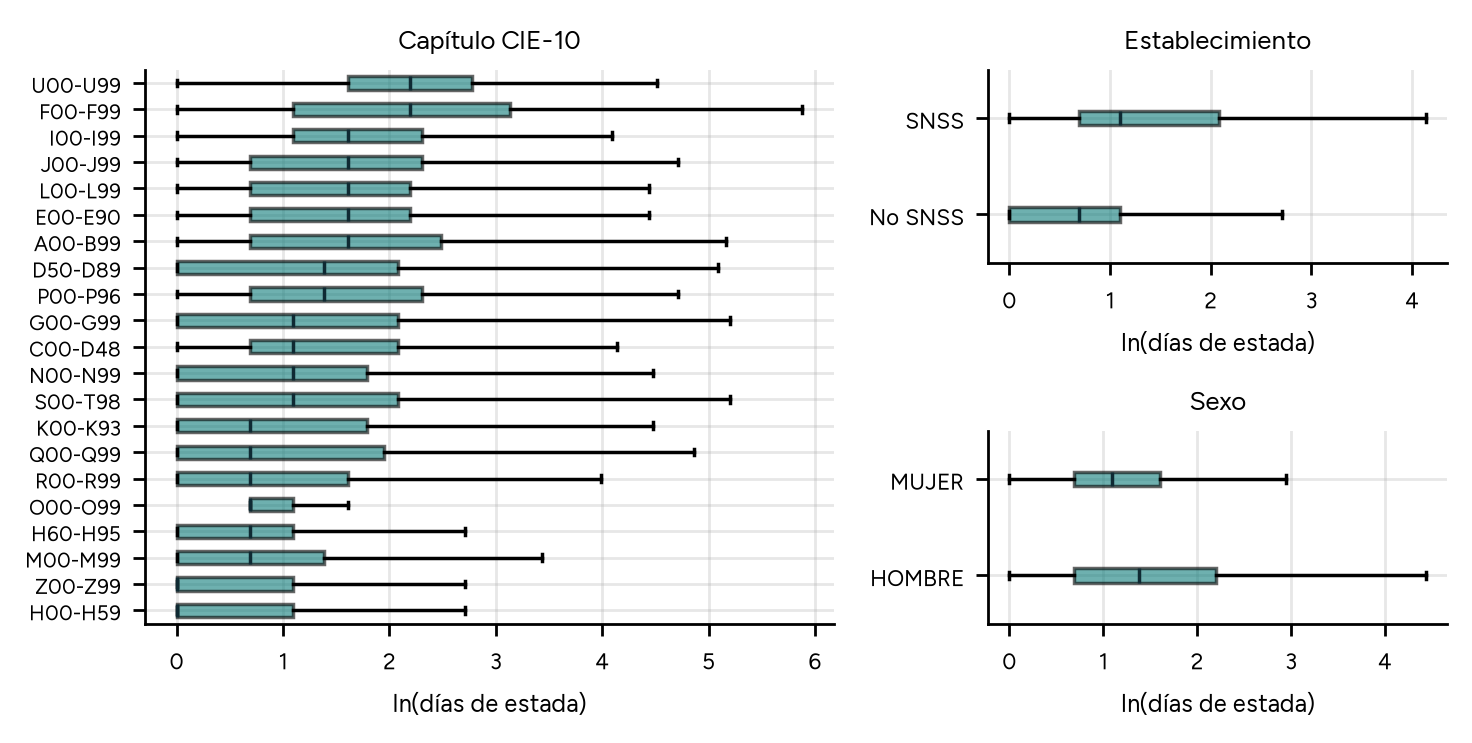
\includegraphics[width=\textwidth]{figs/avance2_bivariado.png}
\caption{Distribución de $\ln$(días) por capítulo \cie{} (ordenado por mediana), por tipo de establecimiento y por sexo. Sin puntos atípicos, para ver las cajas. La mediana de días va de 1 (H00--H59) a 9 (U00--U99).}
\label{fig:biv}
\fuente
\end{figure}

Con casi un millón de egresos, hasta una $V$ de 0,004 sale significativa. Entre las variables explicativas categóricas, la asociación más alta es la de capítulo con cirugía y con sexo ($V=0{,}43$ en ambos; en el sexo por el 100\pct{} de mujeres en O00--O99), seguida de cirugía con establecimiento ($0{,}28$) y de capítulo con condición de egreso ($0{,}26$). Son asociaciones medianas, sin llegar a redundancia (figura~\ref{fig:cramer}).

\begin{figure}[!htb]
\centering
\begin{minipage}[t]{0.49\textwidth}\centering
\captionof{figure}{V de Cramér entre las variables explicativas categóricas.}\label{fig:cramer}
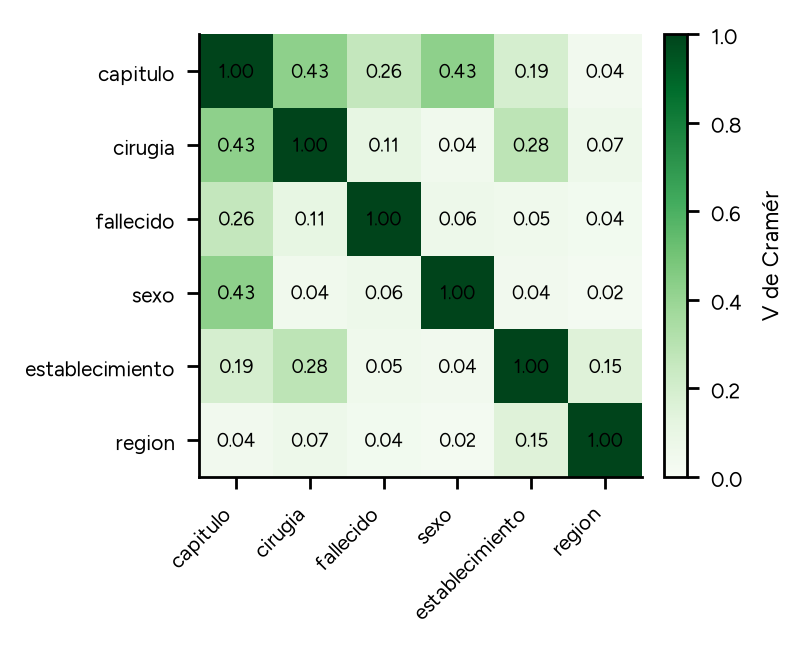
\includegraphics[width=\linewidth]{figs/avance2_cramer.png}
\end{minipage}\hfill
\begin{minipage}[t]{0.49\textwidth}\centering
\captionof{figure}{Media observada de $\ln$(días) por tramo de edad y media ajustada por M3.}\label{fig:edad}
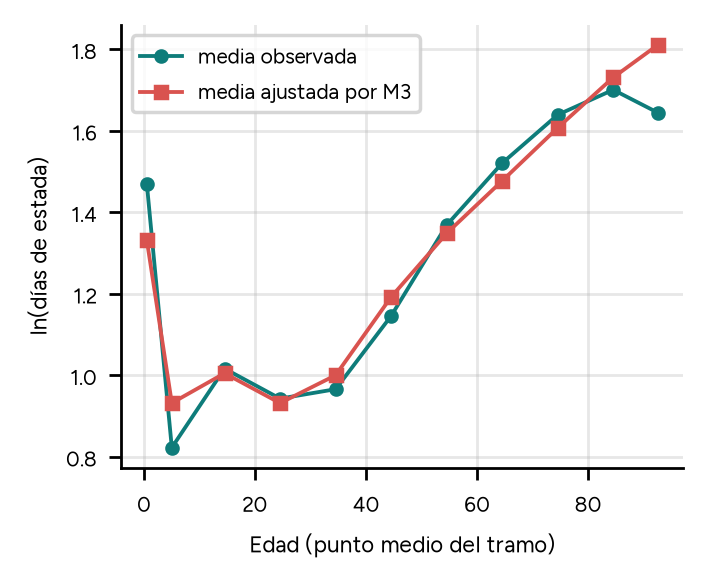
\includegraphics[width=\linewidth]{figs/avance2_edad.png}
\end{minipage}
\fuente
\end{figure}

\subsection{Modelos anidados}

La tabla~\ref{tab:anidados} muestra cuánto cambia el ajuste al incorporar cada bloque. El bloque clínico aporta más: el $R^2$ ajustado pasa de 0 a 0,132 y el BIC baja 137.235. Edad y sexo llevan el $R^2$ ajustado a 0,162, y establecimiento y región a 0,198. Todos los $F$ parciales tienen $p<0{,}001$ y el BIC baja en cada paso. M3 deja sin explicar cerca del 80,2\pct{} de la variación de $\ln$(días).

\begin{table}[!htb]
\centering\small\filas
\caption{Modelos anidados M0 a M3 en la base completa. $k$ es el número de coeficientes.}
\label{tab:anidados}
\begin{tabular}{lrrrrrrr}
\toprule
Modelo & $k$ & $R^2$ aj. & BIC & $\Delta$BIC & $F$ parcial & gl & $\eta^2$ parcial \\
\midrule
M0 & 1 & 0,000 & 2.814.166 & --- & --- & --- & --- \\
M1 & 23 & 0,132 & 2.676.930 & $-137.235$ & 6.717 & 22 & 0,132 \\
M2 & 26 & 0,162 & 2.643.664 & $-33.266$ & 11.295 & 3 & 0,034 \\
M3 & 42 & 0,198 & 2.601.099 & $-42.565$ & 2.734 & 16 & 0,043 \\
\bottomrule
\end{tabular}
\fuente
\end{table}

Como el aporte por bloque depende del orden de entrada, la tabla~\ref{tab:eta} retira cada factor de M3. El capítulo es el factor de mayor aporte ($\eta^2$ parcial $=0{,}074$, efecto mediano), seguido del establecimiento ($0{,}041$) y de la edad ($0{,}035$), ambos pequeños. Con el criterio de 0,01, esos tres son relevantes. Región, sexo, cirugía y condición de egreso son significativos, pero quedan bajo el umbral. Ningún factor solo llega a un efecto mediano en el sentido de 0,06 salvo el capítulo, y el modelo completo llega a 0,198.

\begin{table}[!htb]
\centering\small\filas
\caption{Aporte de cada factor al retirarlo de M3.}
\label{tab:eta}
\begin{tabular}{lrrl}
\toprule
Factor & $R^2$ sin el factor & $\eta^2$ parcial & Efecto (Cohen) \\
\midrule
Capítulo \cie & 0,1339 & 0,0740 & mediano \\
Establecimiento & 0,1638 & 0,0409 & pequeño \\
Edad (edad y edad$^2$) & 0,1692 & 0,0347 & pequeño \\
Región & 0,1942 & 0,0048 & menor que pequeño \\
Sexo & 0,1959 & 0,0026 & menor que pequeño \\
Cirugía & 0,1979 & 0,0002 & menor que pequeño \\
Condición de egreso & 0,1979 & 0,0001 & menor que pequeño \\
\bottomrule
\end{tabular}
\fuente
\end{table}

\subsection{Coeficientes de M3}

La tabla ANOVA del modelo completo da $F=5.830$ con 41 y 968.056 grados de libertad ($p<0{,}001$): la suma de cuadrados de la regresión es 205.399 sobre un total de 1.037.266. La tabla~\ref{tab:coef} muestra los coeficientes principales con su cambio porcentual en la media geométrica de los días. Para el paciente de referencia (mujer, capítulo K00--K93, fuera del SNSS, sin cirugía, vivo, Región Metropolitana y edad media), la media geométrica es de 1,82 días.

\begin{table}[!htb]
\centering\small\filas
\caption{Coeficientes de M3 con error estándar clásico (EE) y robusto a heterocedasticidad (HC3). $\%\Delta=100\,(e^{\beta}-1)$, con intervalo de confianza del 95\pct{} clásico. En la fila de la edad, los errores estándar se muestran con seis decimales.}
\label{tab:coef}
\setlength{\tabcolsep}{4pt}
\begin{tabular}{lrrrr}
\toprule
Factor & $\hat\beta$ (EE) & EE HC3 & $\%\Delta$ & IC 95\pct \\
\midrule
Capítulo F00--F99 (mentales) & 1,147 (0,007) & 0,010 & $+214{,}8$ & 210,4 a 219,3 \\
Capítulo U00--U99 (uso especial) & 0,880 (0,005) & 0,006 & $+141{,}2$ & 138,6 a 143,8 \\
Capítulo P00--P96 (perinatal) & 0,805 (0,007) & 0,009 & $+123{,}8$ & 120,5 a 127,1 \\
Capítulo A00--B99 (infecciosas) & 0,643 (0,007) & 0,009 & $+90{,}3$ & 87,5 a 93,0 \\
Capítulo H00--H59 (ojo) & $-0{,}385$ (0,014) & 0,012 & $-31{,}9$ & $-33{,}7$ a $-30{,}1$ \\
Capítulo Z00--Z99 (factores de contacto) & $-0{,}356$ (0,007) & 0,007 & $-29{,}9$ & $-30{,}9$ a $-28{,}9$ \\
Cirugía & $-0{,}028$ (0,002) & 0,002 & $-2{,}8$ & $-3{,}2$ a $-2{,}3$ \\
Condición de egreso: fallecido & 0,061 (0,005) & 0,007 & $+6{,}3$ & 5,2 a 7,3 \\
Sexo: hombre & 0,107 (0,002) & 0,002 & $+11{,}3$ & 10,9 a 11,8 \\
Establecimiento: SNSS & 0,530 (0,003) & 0,002 & $+70{,}0$ & 69,1 a 70,8 \\
Edad (por año) & 0,009 (0,000048) & 0,000050 & $+0{,}89$ & 0,88 a 0,90 \\
\bottomrule
\end{tabular}
\fuente
\end{table}

Frente al digestivo, los trastornos mentales son el capítulo con mayor aumento y las enfermedades del ojo el de mayor disminución. Los hombres tienen más días que las mujeres con el mismo diagnóstico, edad y establecimiento, como en el Avance 1. Entre regiones, Aisén tiene $-29{,}8\pct{}$ frente a la Región Metropolitana; sin ella el mínimo es $-15{,}8\pct{}$ y el máximo $+0{,}3\pct{}$. Las pruebas $F$ de tipo II rechazan la nulidad de cada factor (capítulo $F=3.867$ con 20 gl; región $F=310$ con 15 gl; establecimiento $F=41.287$), como muestra la figura~\ref{fig:forest}).

La edad se estima con un término lineal y uno cuadrático. A los 74,5 años la media geométrica es 31,1\pct{} mayor que a la edad media. El modelo sigue la subida desde los 20 años y se aparta en los tramos extremos: en menores de un año ajusta 1,33 donde se observa 1,47 (figura~\ref{fig:edad}).

\begin{figure}[!htb]
\centering
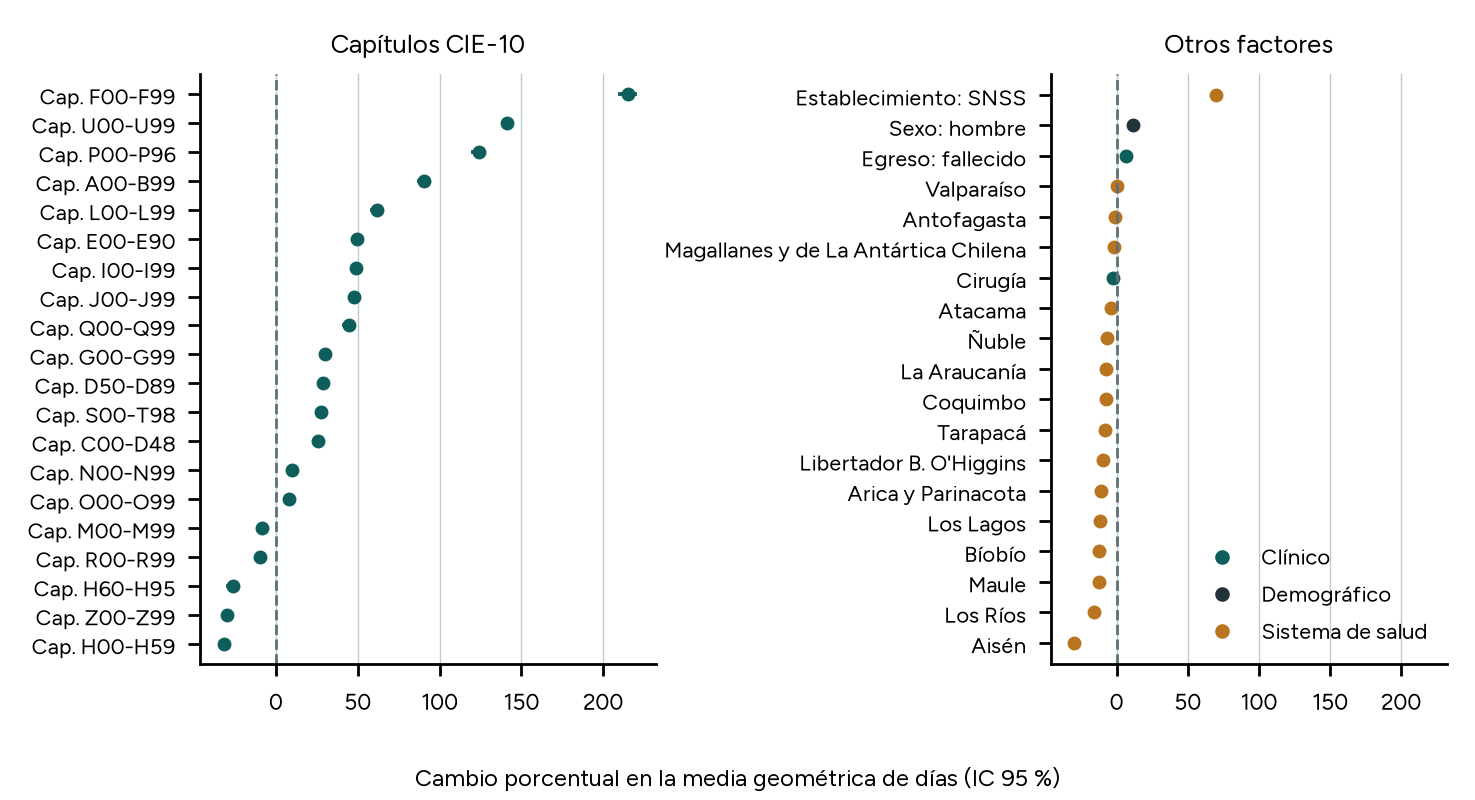
\includegraphics[width=\textwidth]{figs/forest.png}
\caption{Cambio porcentual en la media geométrica ajustada de días asociado a cada coeficiente de M3, con intervalo de confianza del 95\pct{}.}
\label{fig:forest}
\fuente
\end{figure}

\subsection{Ajuste y supuestos}

M3 tiene $R^2=0{,}198$, de modo que cerca del 80\pct{} de la variación de $\ln$(días) queda sin explicar. Al comparar la media geométrica ajustada con la observada por decil de valor ajustado, las diferencias van en ambas direcciones: el decil 10 ajusta 8,05 días frente a 7,40 observados, y el decil 7 ajusta 4,18 frente a 4,56.

\begin{figure}[!htb]
\centering
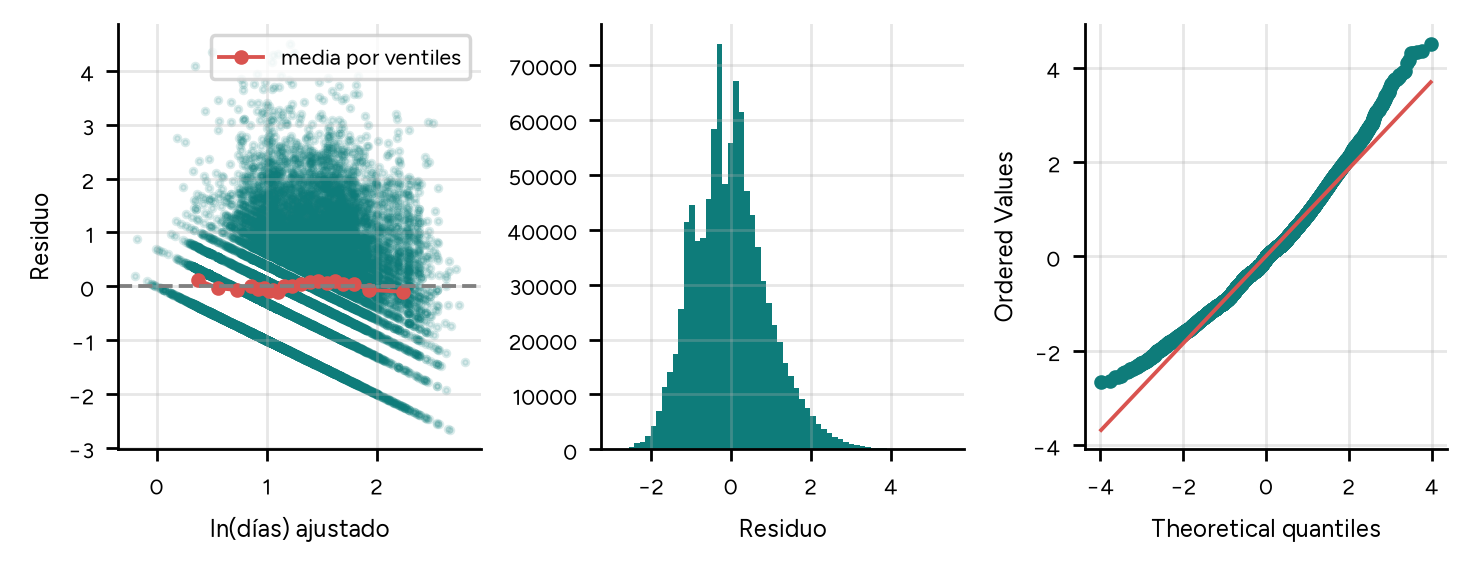
\includegraphics[width=\textwidth]{figs/avance2_residuos.png}
\caption{Residuos frente a valores ajustados (con la media por ventiles), histograma de los residuos y gráfico Q-Q. Se grafica un subconjunto de puntos; las estadísticas usan todos los egresos.}
\label{fig:resid}
\fuente
\end{figure}

Sobre los supuestos: la matriz de diseño tiene rango completo (42 de 42 columnas) y el VIF máximo es 2,36, así que no hay multicolinealidad problemática. La media de los residuos es 0 por construcción del estimador con intercepto, lo que no prueba la exogeneidad. La varianza no es constante: la desviación estándar de los residuos pasa de 0,713 en el primer cuartil del valor ajustado a 1,061 en el cuarto. Los residuos tienen asimetría de 0,492 y curtosis en exceso de 0,542, y el gráfico Q-Q se aparta de la recta en las colas (figura~\ref{fig:resid}). Como los errores estándar clásicos son aproximados, la tabla~\ref{tab:coef} incluye también los robustos HC3. Estos son entre 0,80 y 1,36 veces los clásicos. Ningún coeficiente deja de ser significativo con los errores robustos, y el intervalo que más cambia es el de F00--F99, que pasa de 210,4 a 219,3 con el error clásico a 208,8 a 220,9 con HC3.

\subsection{Sensibilidad a la especificación}\label{sec:sens}

La tabla~\ref{tab:sens} compara M3 con las alternativas. Los 11 tramos de edad (M4) suben el $R^2$ ajustado de 0,198 a 0,202, y la interacción capítulo $\times$ establecimiento (M5) lo lleva a 0,214 con $\eta^2$ parcial de 0,015. Es la única alternativa que pasa el umbral de 0,01. La interacción con la edad (M6) aporta 0,0008. El BIC más bajo es el de M6, pero su aporte es mínimo.

\begin{table}[!htb]
\centering\small\filas
\caption{Especificaciones M3 a M6 en la base completa.}
\label{tab:sens}
\begin{tabular}{lrrrrr}
\toprule
Modelo & $k$ & $R^2$ aj. & $\Delta$BIC & $F$ parcial (gl) & $\eta^2$ parcial \\
\midrule
M3 & 42 & 0,198 & --- & --- & --- \\
M4 (tramos de edad) & 50 & 0,202 & $-4.588$ & 589 (8) & 0,0048 \\
M5 (+ capítulo $\times$ establ.) & 70 & 0,214 & $-14.538$ & 746 (20) & 0,0152 \\
M6 (+ edad $\times$ establ.) & 80 & 0,215 & $-663$ & 80 (10) & 0,0008 \\
\bottomrule
\end{tabular}
\fuente
\end{table}

Al agregar nacionalidad y etnia a M3, el $R^2$ ajustado no cambia (0,19799 frente a 0,19800), el BIC sube 12,6 y el $\eta^2$ parcial es 0,00002; el $F$ parcial es 7,49 ($p=0{,}0006$).

Una selección forward por BIC sobre factores completos llega al mismo modelo M3. Los factores entran en este orden: capítulo, establecimiento, edad, región, sexo, cirugía y condición de egreso, sin descartar ninguno. Los tres primeros (capítulo, establecimiento y edad) ya llevan el $R^2$ ajustado a 0,192.

\subsection{Estadía prolongada: regresión logística}

La prevalencia de estadías prolongadas es 9,39\pct{} (90.909 egresos), y el promedio de la probabilidad ajustada coincide con ella. Cada bloque mejora el ajuste (tabla~\ref{tab:logit}): el pseudo-$R^2$ de McFadden pasa de 0 a 0,106 con los factores clínicos, a 0,121 con edad y sexo y a 0,134 con establecimiento y región, todos con razón de verosimilitud de $p<0{,}001$.

\begin{table}[!htb]
\centering\small\filas
\caption{Modelos logísticos anidados para la estadía prolongada.}
\label{tab:logit}
\begin{tabular}{lrrrrr}
\toprule
Modelo & $k$ & Devianza & Pseudo-$R^2$ & $\chi^2$ (RV) & gl \\
\midrule
L0 (intercepto) & 1 & 603.087 & 0,000 & --- & --- \\
L1 (clínicos) & 23 & 538.998 & 0,106 & 64.089 & 22 \\
L2 (+ edad y sexo) & 34 & 530.221 & 0,121 & 8.777 & 11 \\
L3 (+ establecimiento y región) & 50 & 522.399 & 0,134 & 7.822 & 16 \\
\bottomrule
\end{tabular}
\fuente
\end{table}

Al retirar cada factor de L3, el capítulo vuelve a encabezar el aporte (el pseudo-$R^2$ cae 0,059), seguido de la edad (0,013), el establecimiento (0,010) y la región (0,0048). La condición de egreso (0,0026), el sexo (0,0018) y la cirugía (0,0017) aportan menos de 0,003 cada uno.

La tabla~\ref{tab:or} muestra los OR ajustados. El SNSS tiene un OR de 2,54, la condición de egreso fallecido de 1,76, la cirugía de 1,36 y ser hombre de 1,28. Los trastornos mentales (F00--F99) tienen un OR de 13,0 frente al digestivo, y el embarazo, parto y puerperio (O00--O99) de 0,26. La edad sigue la forma de U que vimos de a pares, con la referencia en 40 a 49 años: el OR sube hasta 1,71 entre los 70 y 79 años, baja a 1,55 entre los 80 y 89 y a 1,15 desde los 90, y es 1,19 en menores de un año.

\begin{table}[!htb]
\centering\small\filas
\caption{Razones de odds ajustadas de L3, con intervalo de confianza del 95\pct{}. Factores binarios, capítulos extremos y tramos de edad.}
\label{tab:or}
\begin{tabular}{lrr}
\toprule
Factor & OR & IC 95\pct \\
\midrule
Establecimiento: SNSS & 2,54 & 2,47 a 2,61 \\
Condición de egreso: fallecido & 1,76 & 1,71 a 1,81 \\
Cirugía & 1,36 & 1,33 a 1,38 \\
Sexo: hombre & 1,28 & 1,26 a 1,30 \\
Capítulo F00--F99 & 13,01 & 12,50 a 13,55 \\
Capítulo O00--O99 & 0,26 & 0,25 a 0,28 \\
Edad: 1 a 9 años & 0,42 & 0,40 a 0,45 \\
Edad: 70 a 79 años & 1,71 & 1,65 a 1,76 \\
Edad: 80 a 89 años & 1,55 & 1,50 a 1,61 \\
Edad: menor de un año & 1,19 & 1,12 a 1,27 \\
\bottomrule
\end{tabular}
\fuente
\end{table}

% =====================================================================
\section{Discusión}

\subsection{Respuesta a la pregunta y contraste de las hipótesis}

El capítulo del diagnóstico, el tipo de establecimiento y la edad son los factores con mayor aporte ajustado a la duración: sus $\eta^2$ parciales son 0,074, 0,041 y 0,035. En la estadía prolongada el diagnóstico también encabeza el aporte, y el SNSS tiene un OR de 2,54. La tabla~\ref{tab:hip} contrasta las hipótesis específicas.

\begin{table}[!htb]
\centering\footnotesize\filas
\caption{Contraste de las hipótesis específicas.}
\label{tab:hip}
\begin{tabularx}{\textwidth}{l Y Y Y}
\toprule
Hipótesis & Duración (lineal) & Prolongada (logística) & Lectura \\
\midrule
$H_{1a}$ clínicos & Capítulo $\eta^2$ parcial 0,074 (mediano). Cirugía y fallecido, 0,0002 y 0,0001 & Capítulo: el pseudo-$R^2$ cae 0,059. Fallecido, OR 1,76 & Se respalda por el capítulo, y por la condición de egreso en la prolongada. La cirugía aporta poco \\
$H_{1b}$ demográficos & Edad: $+0{,}89\pct$ por año, $\eta^2$ 0,035 (pequeño). Sexo, 0,0026 & Edad: cae 0,013 (forma de U). Hombre, OR 1,28 & Se respalda por la edad. El sexo no llega al umbral. Nacionalidad y etnia no aportan \\
$H_{1c}$ sistema de salud & SNSS: $+70{,}0\pct$, $\eta^2$ 0,041 (pequeño). Región, 0,0048 & SNSS, OR 2,54. Región: cae 0,0048 & Se respalda por el establecimiento. La región no llega al umbral \\
\bottomrule
\end{tabularx}
\fuente
\end{table}

\subsection{Relación con la literatura}

El peso del diagnóstico coincide con la lógica de los GRD \citep{fetter1980}. El establecimiento y la edad se mantienen asociados al controlar por diagnóstico, como hallaron \citet{freitas2012} para las estadías extremas dentro de un mismo GRD en Portugal. \citet{olivares2020} también encontró más estadías largas con la edad en Chile, solo en adultos mayores; nuestra logística muestra la misma tendencia sobre los 60 años y además un alza en menores de un año. El $R^2$ de 0,198 es coherente con que el GRD explique buena parte de la duración y aquí solo tengamos el capítulo.

\subsection{Pares frente a modelo conjunto y posibles explicaciones}

Algunas lecturas cambian entre el análisis de a pares y los modelos conjuntos. El establecimiento tenía un efecto despreciable en el chi-cuadrado ($V=0{,}08$), pero al controlar por los demás factores su OR es 2,54. Quizás de a pares lo tapaba la composición de diagnósticos de cada tipo de establecimiento, aunque no lo comprobamos. Cirugía y condición de egreso se achican en el modelo lineal, probablemente porque comparten información con el capítulo ($V=0{,}43$ y $0{,}26$). En la cirugía la dirección difiere entre modelos: los operados tienen una media geométrica de días 2,8\pct{} menor y a la vez más odds de superar 15 días (OR 1,36). Una explicación posible, que no probamos, es que los operados duran menos en general pero tienen una cola larga de complicaciones.

Estas asociaciones no son causales: el SNSS podría concentrar casos más graves, pero la base no trae gravedad para separarlo.

\subsection{Limitaciones}

\begin{itemize}\setlength\itemsep{0pt}
\item La unidad es el egreso, y la base no trae GRD, gravedad, comorbilidades completas ni identificadores de paciente y hospital. Los reingresos y la agrupación por hospital cuestionan la independencia, así que los valores-$p$ y los intervalos pueden quedar optimistas.
\item El filtro de 365 días mantiene la definición del Avance 1 y puede excluir estadías legítimas excepcionalmente largas. No hicimos análisis de sensibilidad a ese umbral.
\item La comparación de especificaciones y la selección previa de variables vuelven exploratoria parte del análisis. Además, 2020 fue el primer año de la pandemia y las asociaciones no se extrapolan automáticamente a otros años.
\end{itemize}

% =====================================================================
\section{Conclusiones}

El diagnóstico, el tipo de establecimiento y la edad son los factores más asociados a cuántos días ocupa un egreso y a que supere los 15 días. Frente a los egresos de otros establecimientos, el SNSS tiene 70,0\pct{} más de media geométrica de días y un OR de 2,54 para la estadía prolongada. Sexo, cirugía, condición de egreso y región son significativos, pero su aporte ajustado es pequeño. La regresión lineal explica el 19,8\pct{} de la variación de $\ln$(días), y las especificaciones alternativas lo llevan como máximo a 21,5\pct{}; el resto depende de gravedad y otras variables que la base no trae.

Los resultados permiten caracterizar qué grupos concentran las estadías largas y orientar preguntas sobre el uso de camas. No permiten atribuir causalidad ni tomar decisiones sobre un paciente individual. Agregar GRD, gravedad e identificadores de paciente y hospital permitiría afinar el papel del establecimiento. Código y cifras: \texttt{avance2\_v7.ipynb} y \texttt{results/cifras\_avance2\_v7.json}.

% =====================================================================
\begin{thebibliography}{99}\small\raggedright\setlength{\itemsep}{0.25em}
\bibitem[Cohen(1988)]{cohen1988} Cohen, J. (1988). \emph{Statistical power analysis for the behavioral sciences} (2.ª ed.). Lawrence Erlbaum Associates.
\bibitem[Fetter et~al.(1980)]{fetter1980} Fetter, R. B., Shin, Y., Freeman, J. L., Averill, R. F., y Thompson, J. D. (1980). Case mix definition by diagnosis-related groups. \emph{Medical Care, 18}(2 Suppl.), 1--53.
\bibitem[Freitas et~al.(2012)]{freitas2012} Freitas, A., Silva-Costa, T., Lopes, F., Garcia-Lema, I., Teixeira-Pinto, A., Brazdil, P., y Costa-Pereira, A. (2012). Factors influencing hospital high length of stay outliers. \emph{BMC Health Services Research, 12}, Artículo 265. \url{https://doi.org/10.1186/1472-6963-12-265}
\bibitem[Kerby(2014)]{kerby2014} Kerby, D. S. (2014). The simple difference formula: An approach to teaching nonparametric correlation. \emph{Comprehensive Psychology, 3}, 11.IT.3.1. \url{https://doi.org/10.2466/11.IT.3.1}
\bibitem[Lequertier et~al.(2021)]{lequertier2021} Lequertier, V., Wang, T., Fondrevelle, J., Augusto, V., y Duclos, A. (2021). Hospital length of stay prediction methods: A systematic review. \emph{Medical Care, 59}(10), 929--938. \url{https://doi.org/10.1097/MLR.0000000000001596}
\bibitem[Lin et~al.(2013)]{lin2013} Lin, M., Lucas, H. C., y Shmueli, G. (2013). Too big to fail: Large samples and the p-value problem. \emph{Information Systems Research, 24}(4), 906--917. \url{https://doi.org/10.1287/isre.2013.0480}
\bibitem[Olivares-Tirado(2020)]{olivares2020} Olivares-Tirado, P. (2020). \emph{Hospitalización social en adultos mayores en el sistema de salud de Chile} [Documento de trabajo]. Superintendencia de Salud. \url{https://www.superdesalud.gob.cl/biblioteca-digital/hospitalizacion-social-en-adultos-mayores-en-el-sistema-de-salud-de-chile/}
\bibitem[Raftery(1995)]{raftery1995} Raftery, A. E. (1995). Bayesian model selection in social research. \emph{Sociological Methodology, 25}, 111--163. \url{https://doi.org/10.2307/271063}
\bibitem[Rodríguez y González(2017)]{rodriguez2017} Rodríguez, D. E., y González, G. J. (2017). \emph{Principios de econometría}. Fondo Editorial ITM.
\bibitem[Schwarz(1978)]{schwarz1978} Schwarz, G. (1978). Estimating the dimension of a model. \emph{The Annals of Statistics, 6}(2), 461--464. \url{https://doi.org/10.1214/aos/1176344136}
\end{thebibliography}
\end{document}
